\documentclass{beamer}

\usepackage[utf8]{inputenc}
\usepackage{booktabs}
\usepackage{xcolor}
%\usetheme{Hannover}
\usecolortheme{crane}
\usepackage{siunitx,cancel}
\usepackage{graphicx}
\usepackage{hyperref}

\usepackage{listings}
\usepackage{color}
\usepackage{xcolor}

%\usepackage[
%backend=biber,
%style=numeric,
%citestyle=numeric,
%sorting=none
%]{biblatex}
%\addbibresource{resources.bib}


% This is the color used for MATLAB comments below
\definecolor{MyDarkGreen}{rgb}{0.0,0.4,0.0}
\definecolor{Blue}{rgb}{0.0,0.0,1.0}
\definecolor{Purple}{rgb}{1.0,0.0,1.0}

\colorlet{mygray}{black!30}
\colorlet{mygreen}{green!60!blue}
\colorlet{mymauve}{red!60!blue}

\lstset{
  backgroundcolor=\color{gray!10},
  basicstyle=\ttfamily,
  columns=fullflexible,
  breakatwhitespace=false,
  breaklines=true,
  captionpos=b,
  commentstyle=\color{mygreen},
  extendedchars=true,
  frame=single,
  keepspaces=true,
  keywordstyle=\color{blue},
  language=c++,
  numbers=none,
  numbersep=5pt,
  numberstyle=\tiny\color{blue},
  rulecolor=\color{mygray},
  showspaces=false,
  showtabs=false,
  stepnumber=5,
  stringstyle=\color{mymauve},
  tabsize=3,
  title=\lstname
}






%\defaultfontfeatures{Scale=MatchLowercase,Mapping=tex-text}
%\setmainfont[Numbers=Lowercase]{Minion Pro}
%\setsansfont[Numbers=Lowercase]{Myriad Pro}
%\setmonofont{Menlo}
%\setmathsfont(Digits,Latin,Greek)[Numbers={Lining,Proportional}]{Minion Pro}

\sisetup{%
  output-decimal-marker = {,},
  per-mode = symbol,
  %round-mode = places,
  %round-precision = 5
}

\DeclareSIUnit \electronvolt {\ensuremath{eV}}
\DeclareSIUnit \lightspeed {\ensuremath{c}}
\DeclareSIUnit \dalton{\ensuremath{u}}
\DeclareSIUnit \echarge{\ensuremath{e}}


\newcommand{\mvec}[2]{
\ensuremath{\left(
\begin{array}{c}
#1\\
#2\\
\end{array}
\right)}
}

\newcommand{\Span}{\ensuremath{\mathrm{Span}}}
\newcommand{\Mat}{\ensuremath{\mathrm{Mat}}}
\newcommand{\R}{\ensuremath{\mathbb{R}}}
\newcommand{\Rno}{\ensuremath{\mathbb{R}\backslash\{0\}}}
\newcommand{\Z}{\ensuremath{\mathbb{Z}}}
\newcommand{\ol}[1]{\ensuremath{\overline{#1} } }
\newcommand{\F}[1]{\ensuremath{\mathbb{F}_{#1} } }


%Information to be included in the title page:
\title{Exploring electric and magnetic forces using computer simulations}
\author{Nikolaj Roager Christensen}
\institute{Student Colloquium in Physics and Astronomy, Aarhus University}
\date{March 2021}

%\AtBeginSection[]
%{
%}

\titlegraphic
{
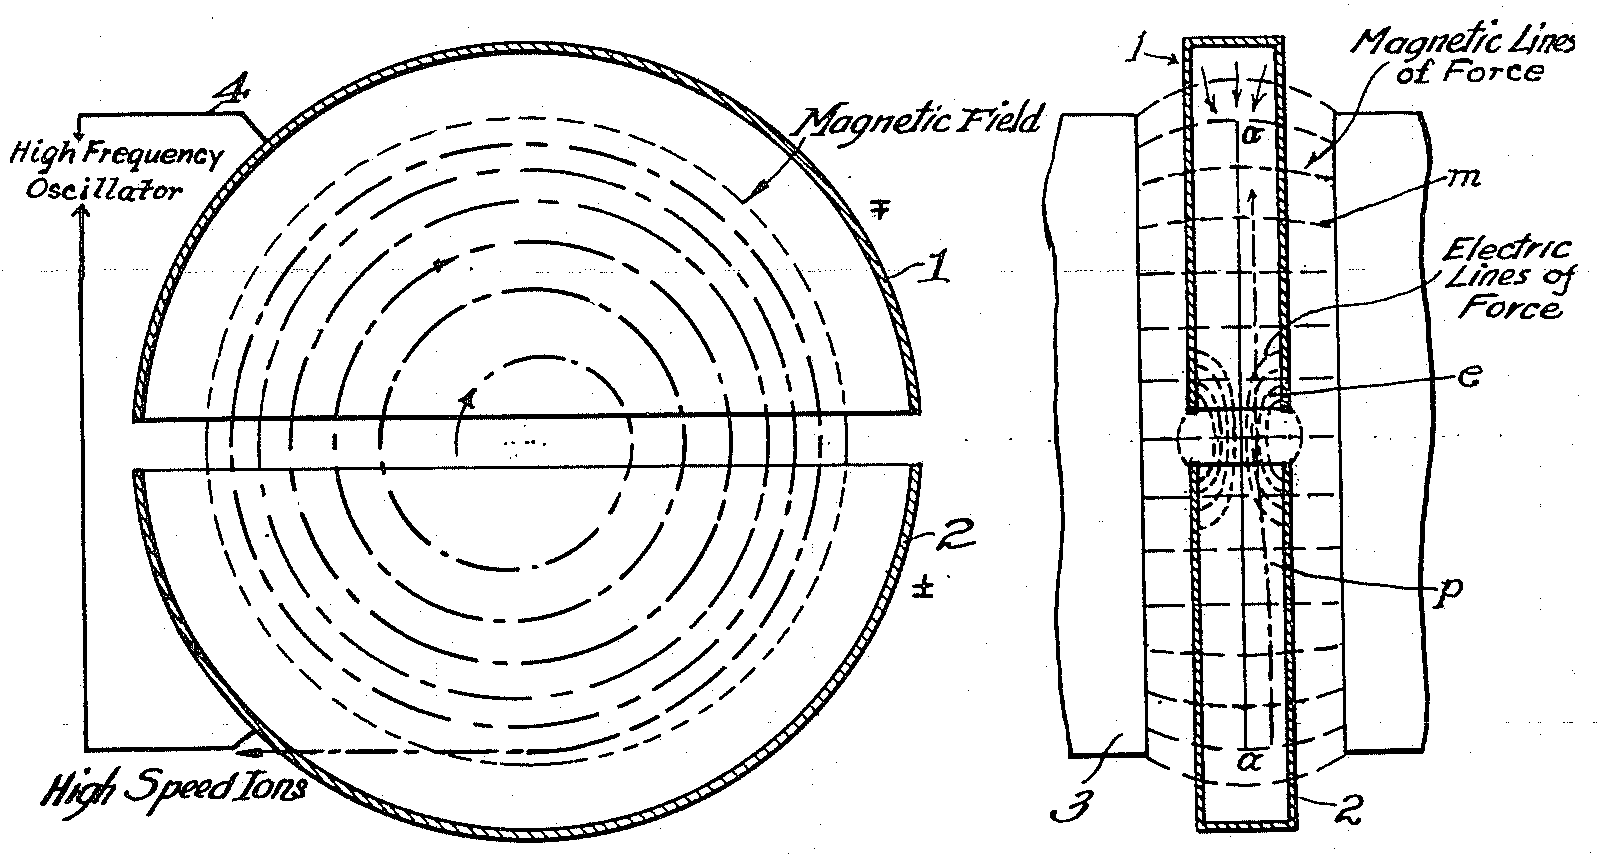
\includegraphics[width=0.5\textwidth]{Cyclotron_patent.png}
}
\begin{document}

\frame{\titlepage}



\section{introduction (5 min)}

\begin{frame}
\frametitle{Wellcome}

\begin{itemize}
\item<1-> Todays topic: particles in electric and magnetic fields
\item<2-> Explored using computer-simulations
\item<3-> Todays plan
\end{itemize}

 \visible<3->{%
\tableofcontents[currentsection]
}
\end{frame}


\begin{frame}
\frametitle{Introduction, what and why}
\begin{columns}
\begin{column}{0.5\linewidth}
\begin{itemize}
\item<1-> (Classical) Charged particles in Electric and Magnetic fields
\item<2-> How can magnetic fields steer and collect particles
\item<3-> Real world examples:
\begin{itemize}
\item<3-> Magnetic traps: ``Tokamak" style fusion reactors.
\item<5-> Particle accelerators, here cyclotron.
\item<6-> The Aurora.
\end{itemize}
\end{itemize}
\end{column}
\begin{column}{0.5\linewidth}
\only<3>{
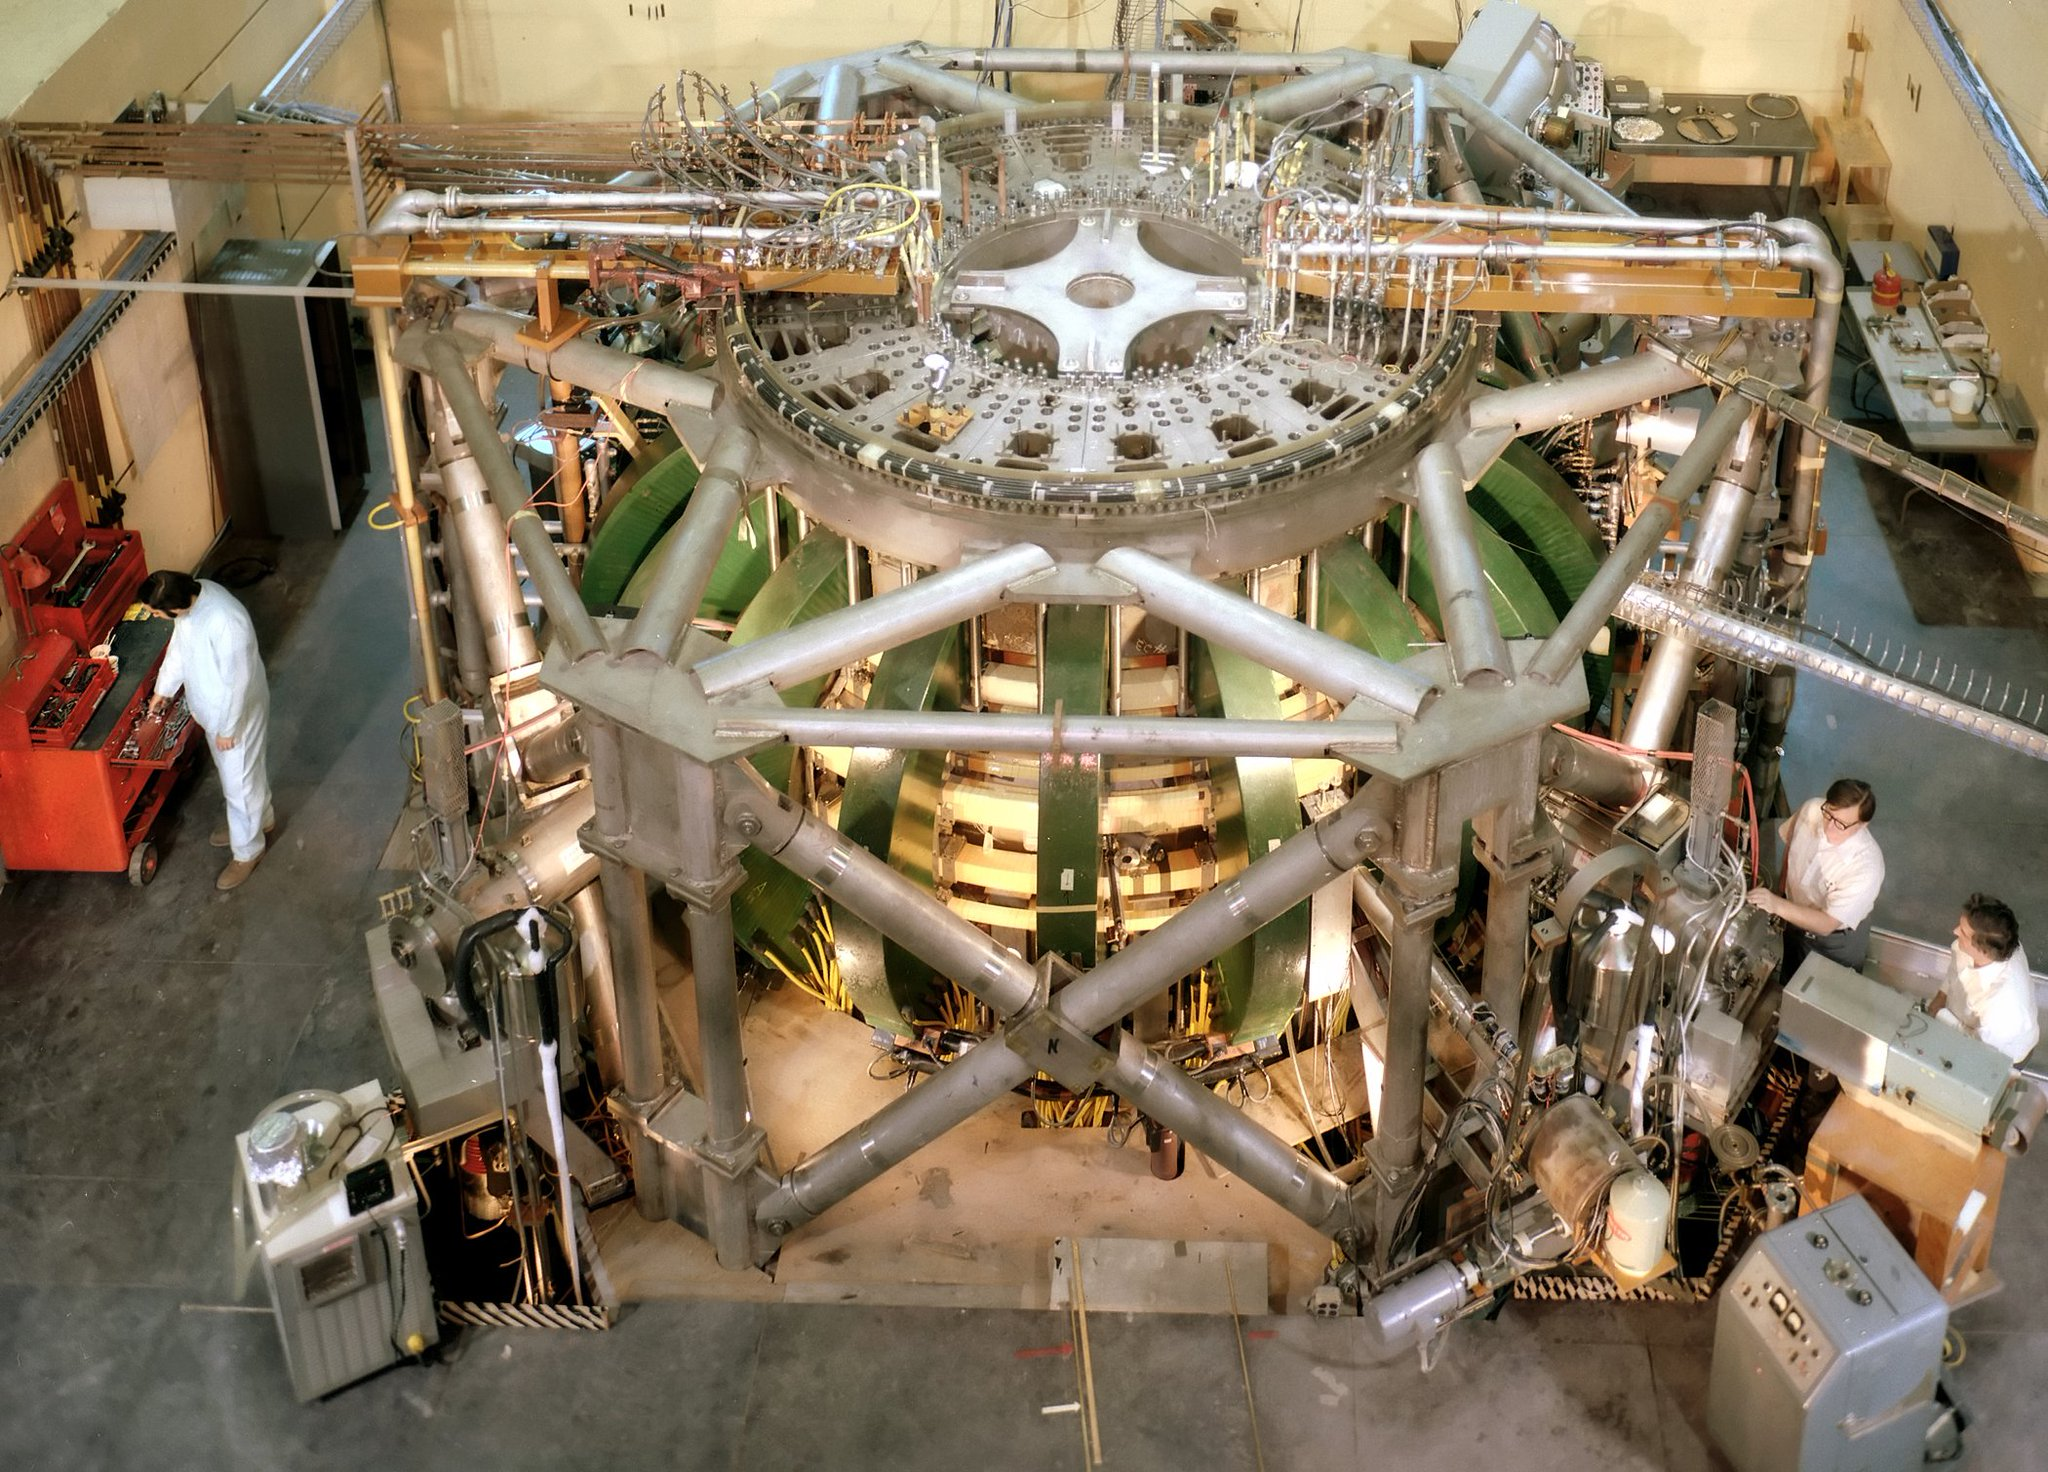
\includegraphics[width=\linewidth]{Princeton_Large_Torus_1975.jpg}

{\color{gray} Princeton Large Torus in 1975, image in Public Domain}
}%
\only<4>{
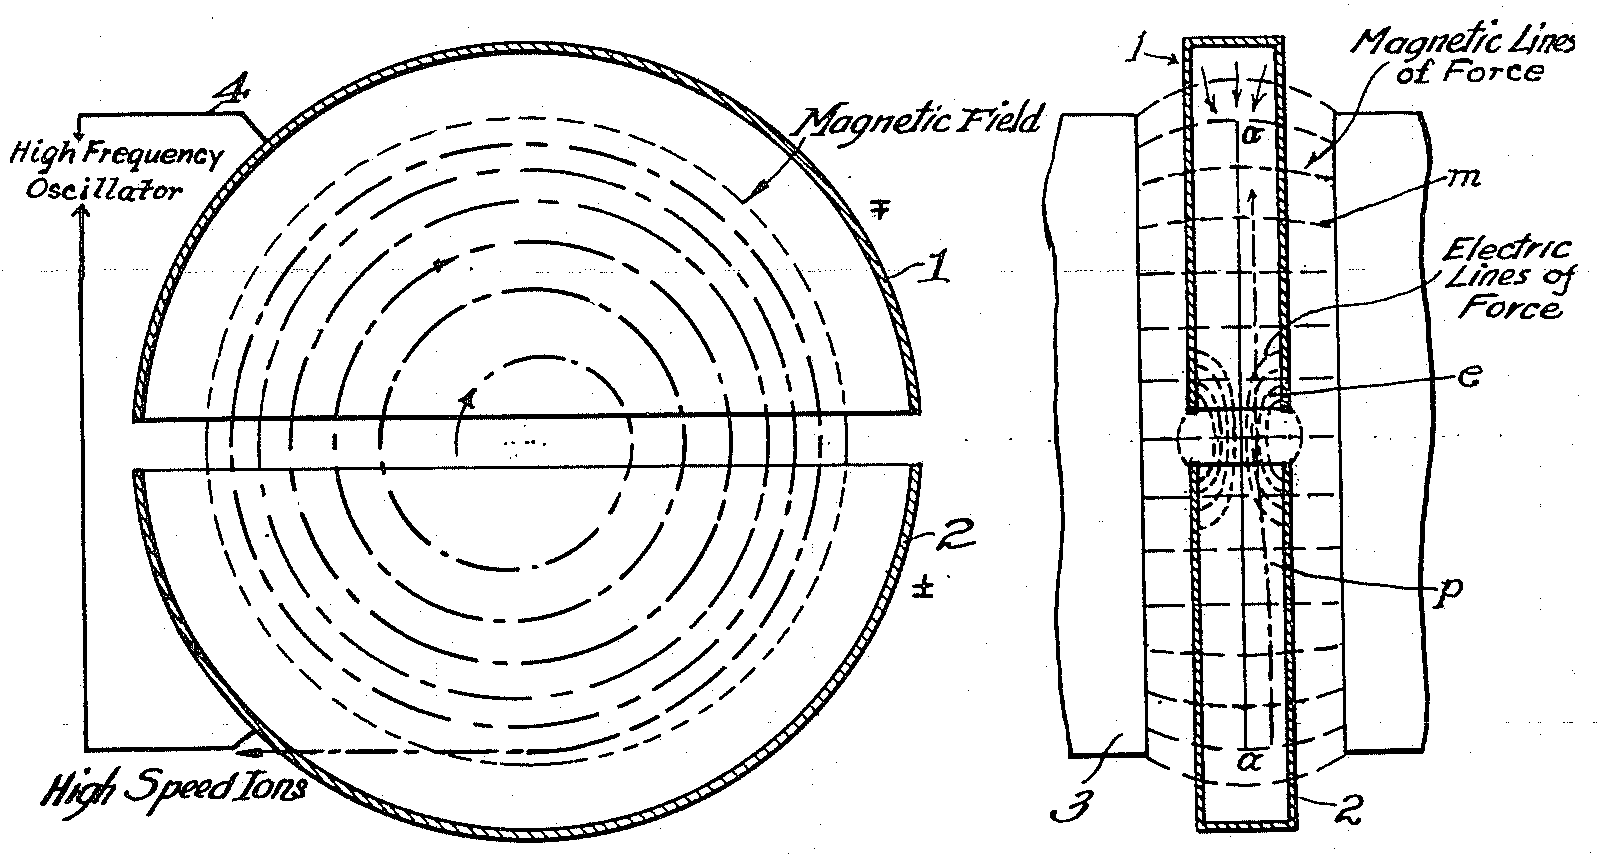
\includegraphics[width=\linewidth]{ Cyclotron_patent.png}


{\color{gray} Ernest O. Lawrence, 1934, U.S. Patent 1,948,384; image in Public Domain}
}%
\only<5>{
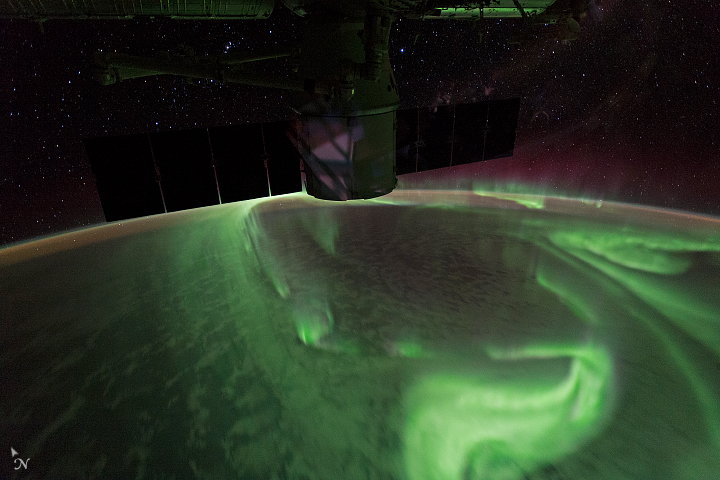
\includegraphics[width=\linewidth]{Aurora_australis_ISS.jpg}

{\color{gray} Nasa: Aurora Australis, Indian Ocean from ISS in 2017; image in Public domain}
}
\end{column}
\end{columns}
\end{frame}


\begin{frame}
\frametitle{How: Numeric-simulation}
\begin{itemize}
\item<1-> When analytical solutions are not practical.
\item<2-> Testing experimental setups.
\item<3-> Here, the \lstinline{odeint} library in C++.
\begin{itemize}
\item<5-> Runge Kutta Algorithm
\item<5-> Identical to \lstinline{odeint}/\lstinline{ode45} in scipy or matlab.
\item<6-> Need an ODE: $\dot{\vec{x}}=f(\vec{x},t)$.
\end{itemize}
\item<4-> Not the main focus.
\item<7-> Simulations are not experiments!
\end{itemize}
\end{frame}

\section{Theory and setup (5 minutes)}

\begin{frame}
\frametitle{Theory and setup (5 minutes)}
\tableofcontents[currentsection]
\end{frame}



\begin{frame}
\frametitle{Theory: Electric and magnetic fields}
\begin{itemize}
\item<1-> Some repetition from Electrodynamics
\item<2-> The Lorentz force:

\only<2-3>{%
\begin{equation*}
\vec{F} = q ( \vec{v}\times \vec{B}+\vec{E}).
\end{equation*}
}
\only<4->{%
\begin{align*}
m \ddot{\vec{r}} &= q ( \dot{\vec{r}}\times \vec{B}+\vec{E}).
\end{align*}
}

\item<3-> $\vec{E}(\vec{r},t)$ and $\vec{B}(\vec{r},t)$.

\item<4-> Only 1 particle! so pre-programmed depending on the setup.
\end{itemize}
\end{frame}

\begin{frame}
\begin{itemize}
\frametitle{Theory: Alternative approach}

\item<1-> I used:

\begin{align*}
m \ddot{\vec{r}} &= q ( \dot{\vec{r}}\times \vec{B}+\vec{E}).
\end{align*}

\item<2-> Other options exists: potentials

\begin{align*}
\vec{E}(\vec{r},t) &= \nabla \phi(\vec{r},t)\\
\vec{B}(\vec{r},t) &= \nabla \times \vec{A}(\vec{r},t)
\end{align*}

\item<3-> Hamiltonian equation* of motion

\begin{align*}
\dot{r_i} &= \frac{\partial \mathcal{H}}{\partial p_i},\\
\mathcal{H} &= \frac{\vec{p}^2}{2m}+V(\vec{r}) \rightarrow \frac{(\vec{p}^2-q\vec{A}(\vec{r},t))}{2m}+q\phi(\vec{r},t)+V(\vec{r}).
\end{align*}

\end{itemize}
\end{frame}

\begin{frame}[fragile]
\frametitle{The ODE implementation}
%\only<1>{%
\begin{lstlisting}
auto ODE = [...](const state_type Data, state_type &dDatadt, const double t)
{
    //Extract position and velocity from data
    ...

    //Get current force
    vec F = Charge*(Fields.get_Efield(pos,t)+
        cross(velocity,Fields.get_Bfield(pos,t)));

    vec dVdt = F*Inv_mass;  //get acceleration

    //Save derivative of data
    ...
};
\end{lstlisting}
\end{frame}


\begin{frame}
\frametitle{Known results, cyclotron motion $\vec{B}$ fields}
\begin{columns}
\begin{column}{0.5\linewidth}
\begin{itemize}
\item<1-> Magnetic forces do no work:

\only<2>
{
\begin{equation*}
dW_{\vec{B}}= \vec{F}_B \cdot d\vec{r}\propto (\vec{v}\times \vec{B})\cdot \vec{v} = 0.
\end{equation*}
}

\item<3-> Cyclotron motion ($\vec{v}=\vec{v}_\perp+\vec{v}_\parallel$):

\only<4>
{
\begin{equation*}
|\vec{F}_B| = |q ( \vec{v}\times \vec{B})| =|q| |v_{\perp}| |B|.
\end{equation*}
}
\item<4-> Same as Centripetal force

\item<5> Cyclotron radius and frequency:

\begin{equation*}
R = \frac{v_\perp m}{|q|B} \quad \omega_c =\frac{|q|B}{m}.
\end{equation*}

\end{itemize}
\end{column}
\begin{column}{0.5\linewidth}
\only<1-2>{%
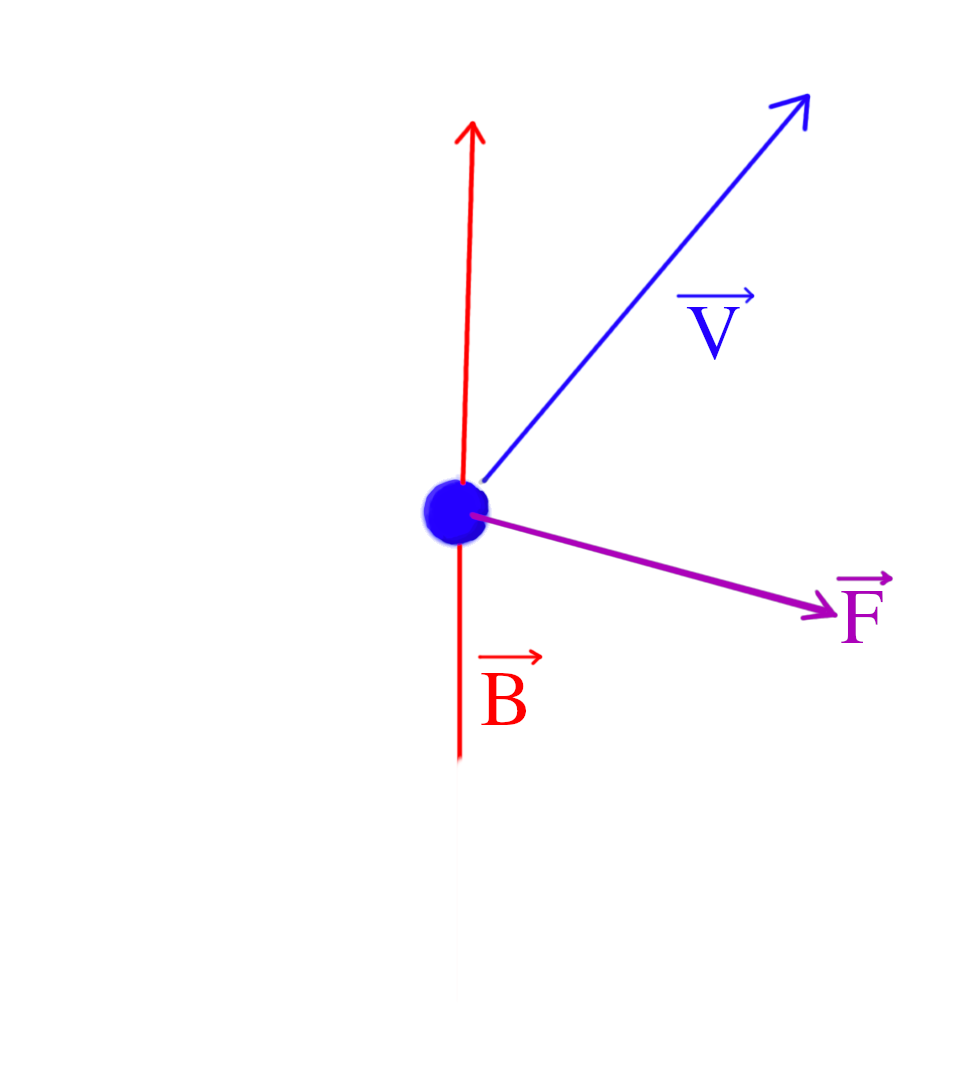
\includegraphics[width=\linewidth]{dw0.png}}%
\only<3>{%
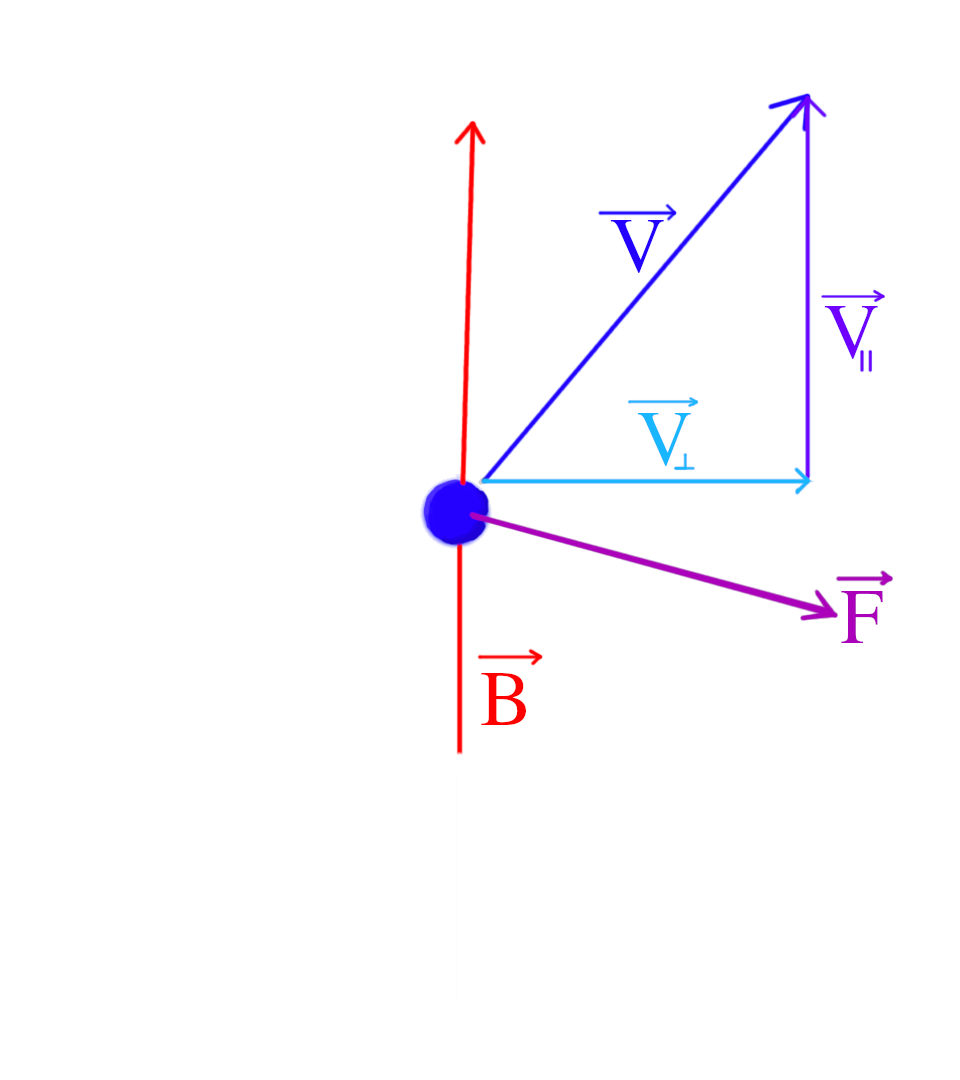
\includegraphics[width=\linewidth]{cyc0.png}}%
\only<4->{%
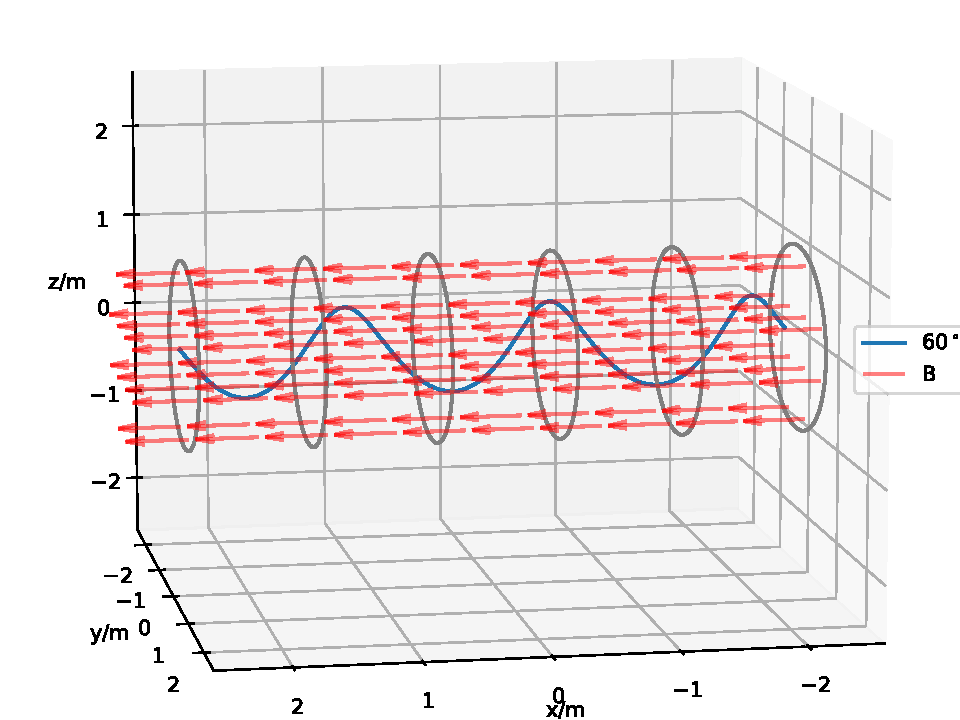
\includegraphics[width=\linewidth]{helix.pdf}
\end{column}
\end{columns}
\end{frame}

\section{Simulations}

\begin{frame}
\frametitle{Protons in a Solenoid}
\begin{columns}
\begin{column}{0.5\linewidth}
\begin{itemize}

\item<1-> Solenoid with $N=1000$ turns per $m$, $I=\SI{5}{\ampere}$, $r=\SI{1}{\meter}$

\begin{align*}
\vec{B}=\mu_0 N I \vec{\hat{x}}.
\end{align*}

\item<2-> Proton with $E_{kin}=\SI{1}{\mega\electronvolt\per\square\lightspeed}$ ($|v|\approx \SI{3.195E5}{\meter\per\second}$)


\begin{equation*}
R \approx \SI{0.5}{\meter}\sin(\theta) \quad T=\frac{2\pi}{\omega} \approx \SI{1.7}{\micro\second}
\end{equation*}

\end{itemize}
\end{column}
\begin{column}{0.5\linewidth}
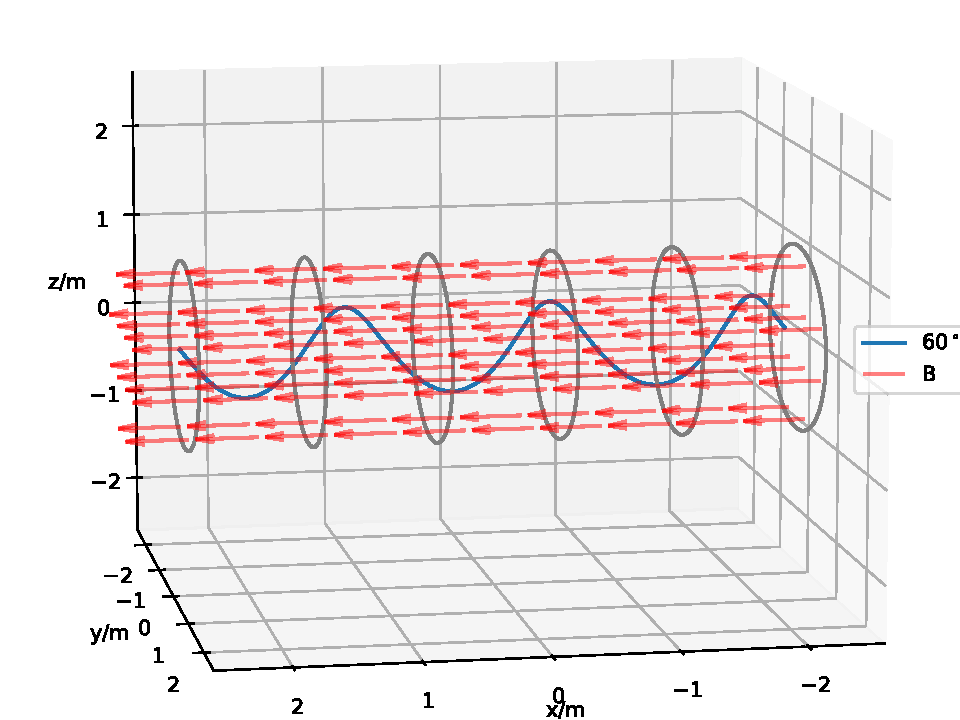
\includegraphics[width=\linewidth]{helix.pdf}
\end{column}
\end{columns}
\end{frame}

\begin{frame}
\frametitle{Protons in a Solenoid, 3D plots}
\only<1>{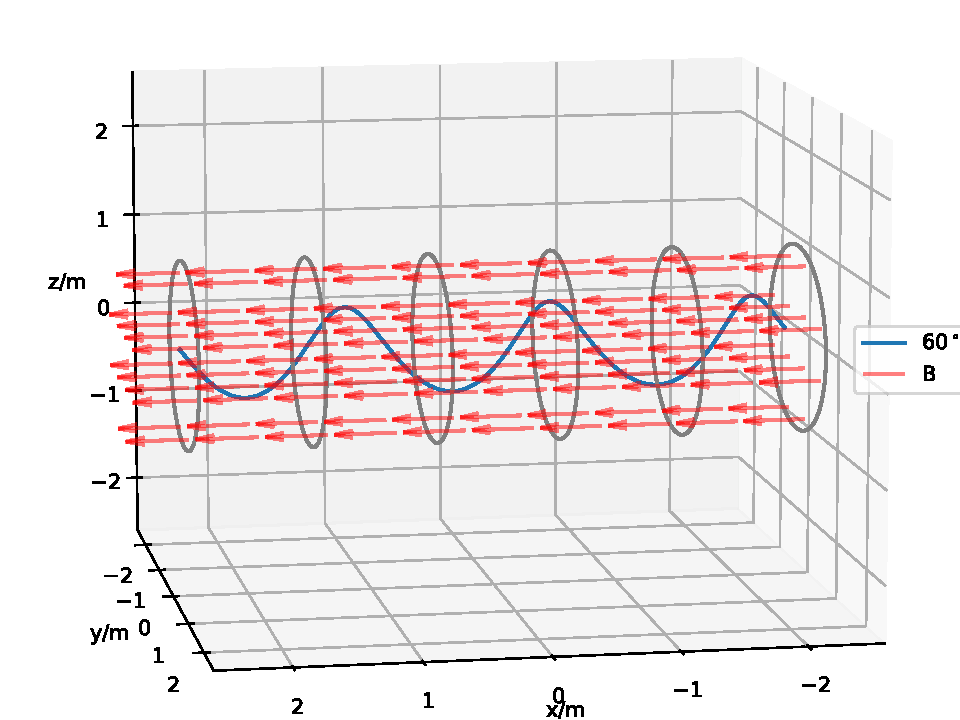
\includegraphics[width=\linewidth]{helix.pdf}}%
\only<2>{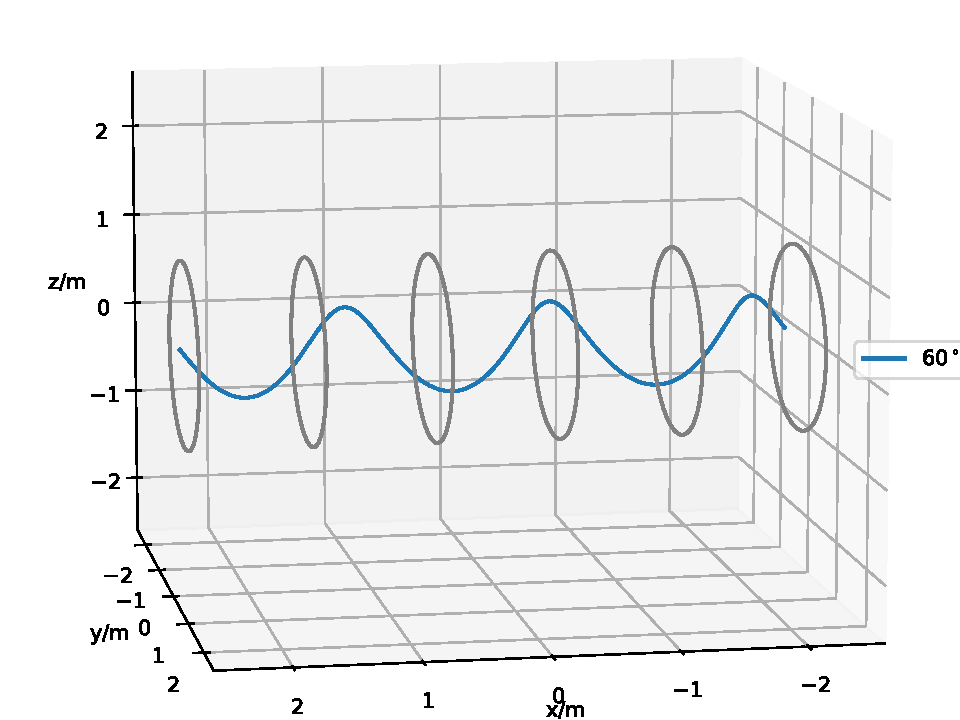
\includegraphics[width=\linewidth]{helix1.pdf}}%
\only<3>{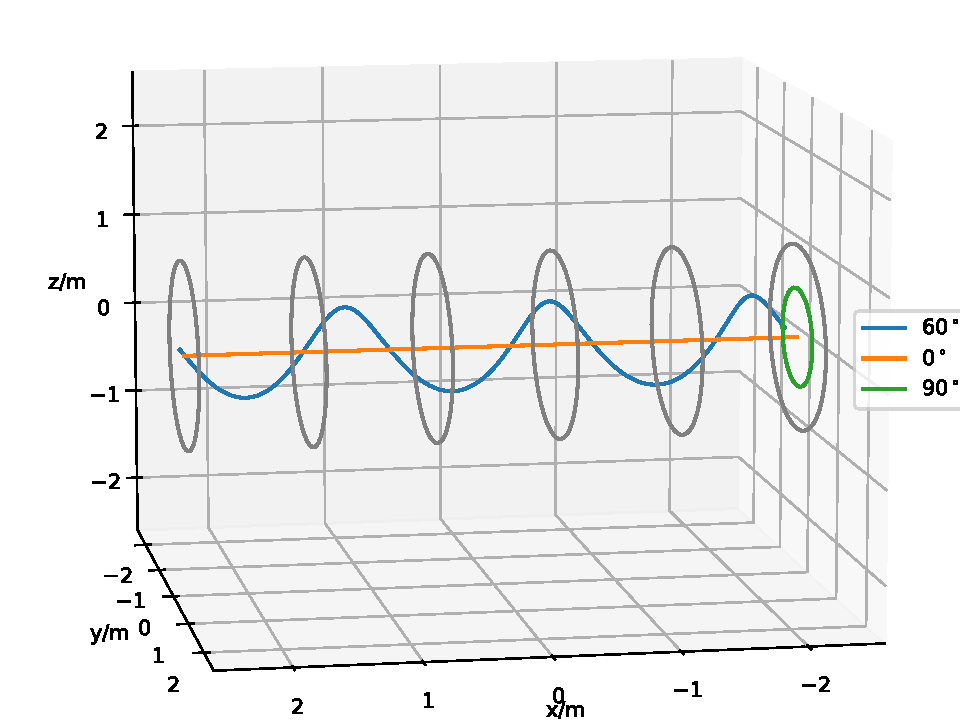
\includegraphics[width=\linewidth]{solenoid_3D0.pdf}}%
\only<4>{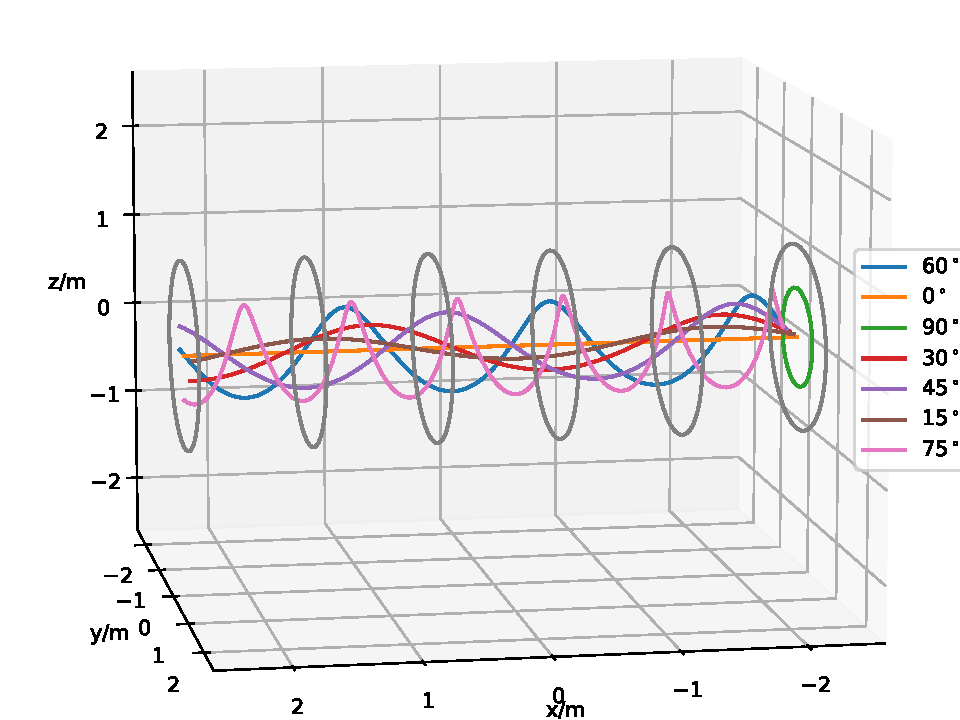
\includegraphics[width=\linewidth]{solenoid_3D1.pdf}}%
\end{frame}


\begin{frame}
\frametitle{Protons in a Solenoid, 2D plots}
\only<1>{%
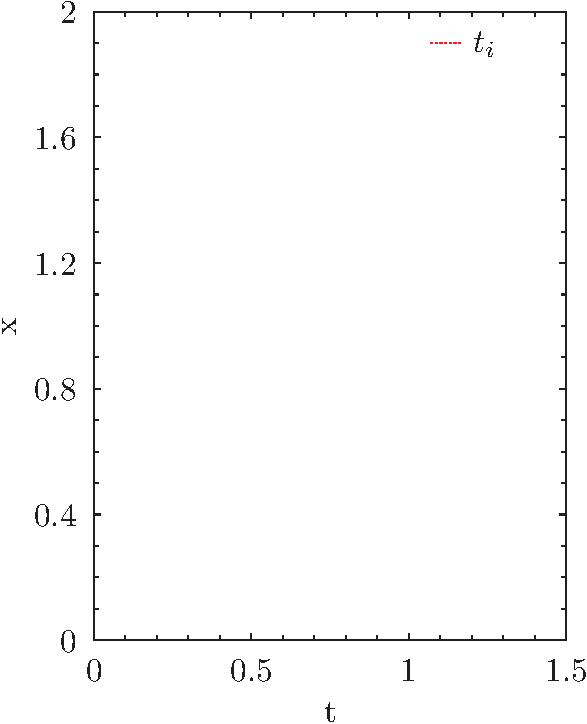
\includegraphics[width=0.66\linewidth]{solenoid_xz_view1.pdf}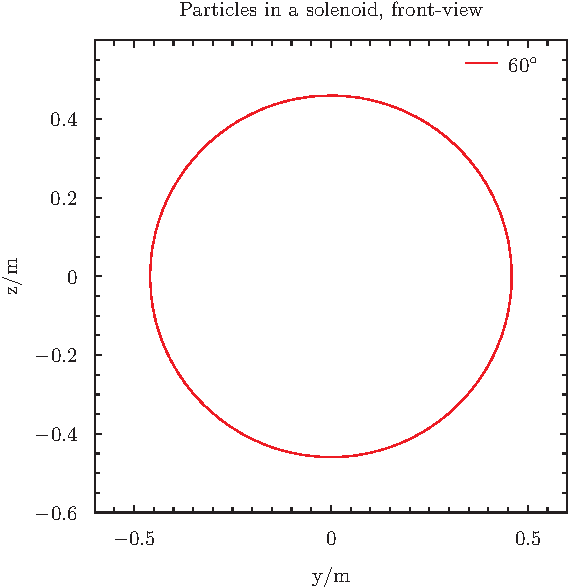
\includegraphics[width=0.33\linewidth]{solenoid_yz_view1.pdf}}%
\only<2>{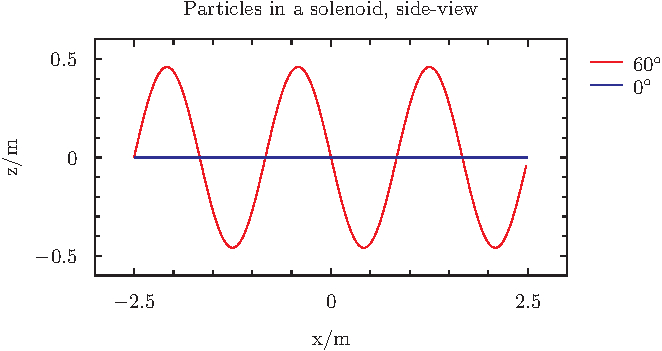
\includegraphics[width=0.66\linewidth]{solenoid_xz_view2.pdf}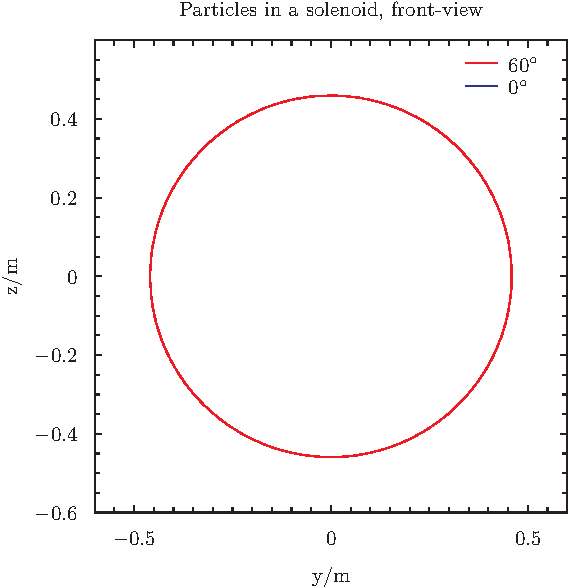
\includegraphics[width=0.33\linewidth]{solenoid_yz_view2.pdf}}%
\only<3>{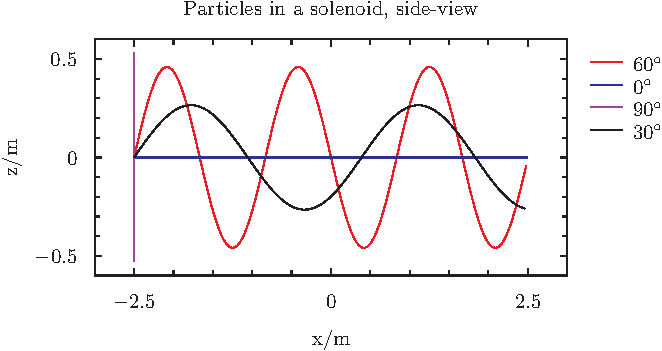
\includegraphics[width=0.66\linewidth]{solenoid_xz_view3.pdf}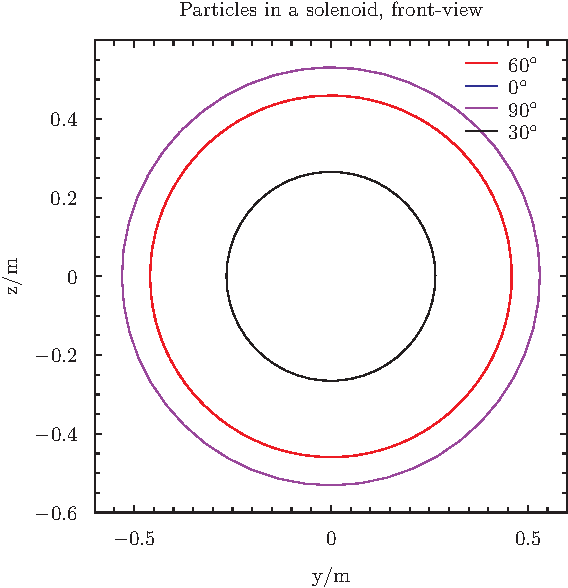
\includegraphics[width=0.33\linewidth]{solenoid_yz_view3.pdf}}%
\only<4>{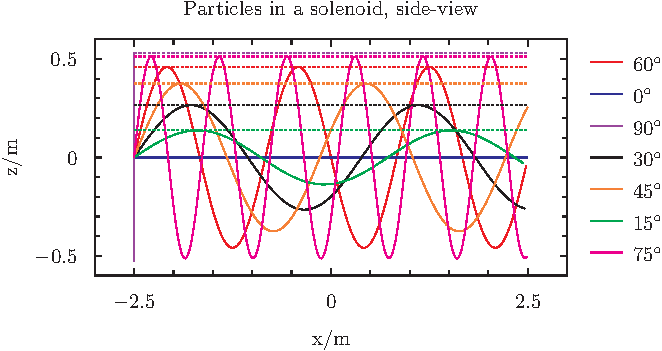
\includegraphics[width=0.66\linewidth]{solenoid_xz_view4.pdf}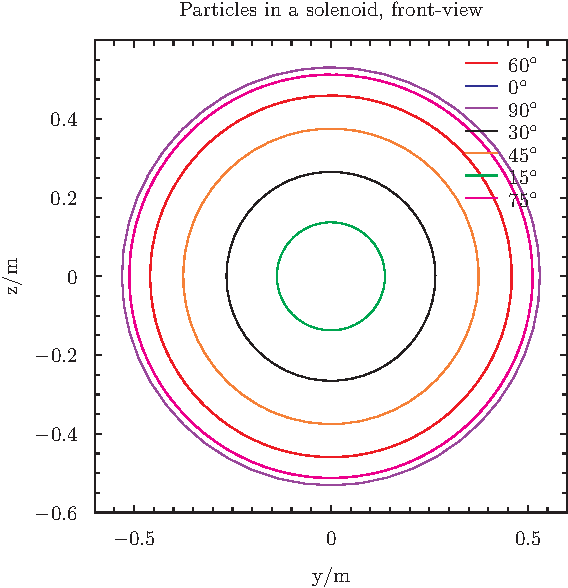
\includegraphics[width=0.33\linewidth]{solenoid_yz_view4.pdf}}%
\only<5>{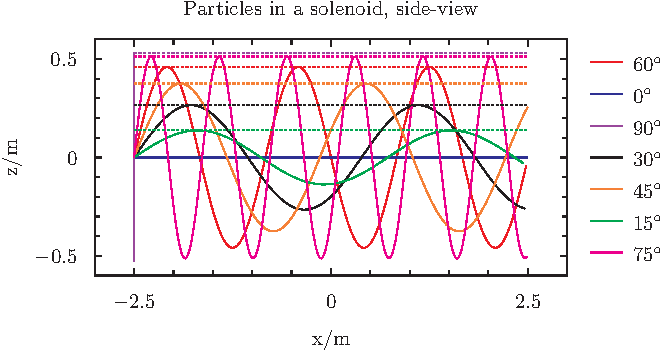
\includegraphics[width=0.66\linewidth]{solenoid_xz_view5.pdf}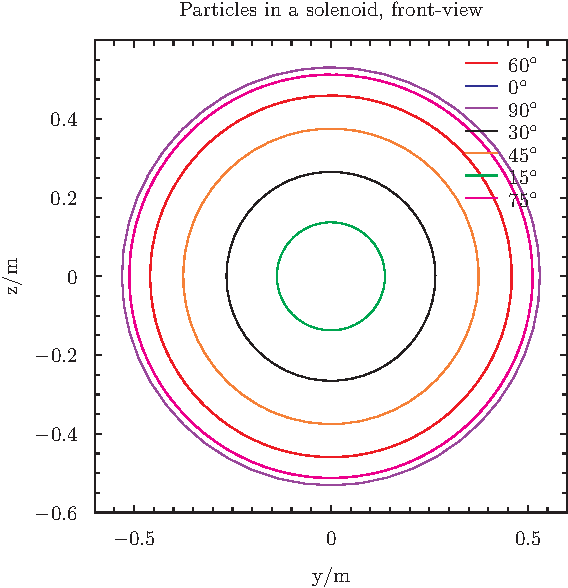
\includegraphics[width=0.33\linewidth]{solenoid_yz_view4.pdf}}%
\end{frame}


\begin{frame}
\frametitle{Sanity check, no work}
\only<1>{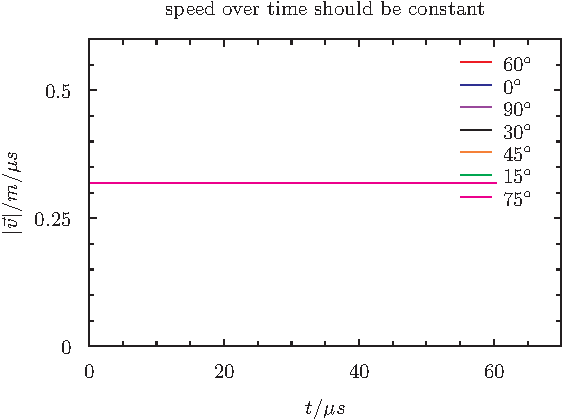
\includegraphics[width=\linewidth]{solenoid_speed1.pdf}}%
\only<2>{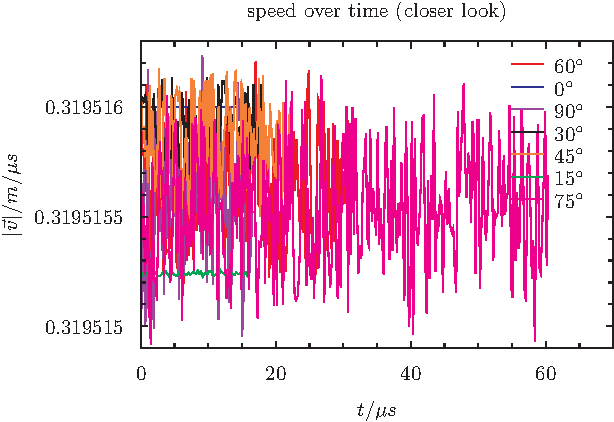
\includegraphics[width=\linewidth]{solenoid_speed2.pdf}}%
\end{frame}


%Electric and magnetic fields
%The Lorentz force
%Newtons 2nd law, ordinary differential equation*
%Alternative, electric and magnetic potentials

\end{document}

%\printbibliography



1 kg = 6.0221412901167394e+26  u
1 C  = 6.241509074460763e+18  e
1 s  = 1000000.0  μs
1 T  = 96.48534061671654  kg/(μs e)

m_p  = 1.672621911e-27 kg  1.0072765472987066  u
q_p  = 1.602176634e-19 C  1.0  e

v  = 319515.54756336455 m/s  0.31951554756336453  m/(μs)
ω  = 601855.8420197117  1/s  0.6018558420197118  1/(μs)
T  = 1.6615274459149445e-06  s  1.6615274459149445  (μs)
r  = 0.5308838516730721  m  0.5308838516730721  m
B  = 0.006283185307179587  T  0.6062352745211712  kg/(μs e)

\frametitle{Sketch: content plan (1/2)}
What "chapters" do I have, and how long do I want to spend on each, I will prefer if questions are permitted during the presentation

\begin{itemize}
\item Introduction (5 minutes)

\item Background, electric and magnetic fields, the Lorentz-force (5 minutes)

\end{itemize}
\end{frame}
\begin{frame}
\frametitle{Sketch: content plan (2/2)}
\begin{itemize}
\item Testing the simulation, the solenoid: cyclotron motion, conservation of energy (5 min)

\item Curved magnetic fields: Tokamak fusion reactors (5 min).

\item Electric fields, the Cyclotron accelerator (8 minutes)

\item The Aurora and the Earth magnetic field (8 minutes)

\item Outlook, relativistic particles (if time permits)

\item Questions (Remaining time)

\end{itemize}
\end{frame}
